% Gerado automaticamente por GeradorListaPDF — não editar manualmente
\documentclass[12pt]{article}
\usepackage{pratiqueja}
\usepackage{tabularray}
\usepackage{cancel}
\definecolor{iris}{rgb}{0.39, 0.44, 1}
\definecolor{babypink}{rgb}{1, 0.42, 0.52}

\newcommand{\numex}[1]{%
  \begin{tcolorbox}[enhanced,arc=3pt,boxrule=0pt,colback=rulebg,colframe=rulebg,left=4pt,right=4pt,top=1pt,bottom=1pt,nobeforeafter,on line]{\bfseries\small\color{darkblue}#1}\end{tcolorbox}\hspace{4pt}}
\newcommand{\altline}[2]{%
  \def\altph{---}%
  \def\altarg{#2}%
  \ifx\altarg\altph\else
    \noindent{\bfseries\color{darkblue}\small(#1)}~{\small#2}\par
  \fi}
\newlength{\cellheight}
\setlength{\cellheight}{11.7cm}
\newcommand{\alts}[5]{%
  \altline{A}{#1}%
  \altline{B}{#2}%
  \altline{C}{#3}%
  \altline{D}{#4}%
  \altline{E}{#5}
  \vspace{0.3cm}}
\newcommand{\ex}[7]{%
  \parbox[t][\cellheight][t]{\linewidth}{%
    \setlength{\parskip}{6pt}%
    \noindent\numex{#1}{\small\color{bodytext}#2}\par\vfill
    \alts{#3}{#4}{#5}{#6}{#7}}}
\newcommand{\exImg}[8]{%
  \parbox[t][\cellheight][t]{\linewidth}{%
    \setlength{\parskip}{6pt}%
    \noindent\numex{#1}{\small\color{bodytext}#2}\par
    {\centering #3\par}%
    \vfill
    \alts{#4}{#5}{#6}{#7}{#8}}}
\newcommand{\exd}[2]{%
  \parbox[t][\cellheight][t]{\linewidth}{%
    \setlength{\parskip}{6pt}%
    \noindent\numex{#1}{\small\color{bodytext}#2}}}
\newcommand{\resheader}[2]{%
  \begin{tcolorbox}[enhanced,arc=3pt,boxrule=0pt,colback=rulebg,colframe=rulebg,left=4pt,right=4pt,top=1pt,bottom=1pt,nobeforeafter,on line]{\bfseries\small\color{darkblue}#1\hspace{5pt}{\color{mutedtext}\tiny\textbullet}\hspace{5pt}\color{vegreen}#2}\end{tcolorbox}\hspace{4pt}}
\newcommand{\res}[3]{%
  \noindent\resheader{#1}{#2}\hspace{0.3cm}{\fontsize{10}{12}\selectfont\setlength{\lineskip}{6pt}\setlength{\lineskiplimit}{2pt}\setlength{\jot}{8pt}\color{bodytext}#3\par}\vspace{0.4cm}}
\newcommand{\resd}[2]{%
  \noindent\numex{#1}\hspace{0.3cm}{\fontsize{10}{12}\selectfont\setlength{\lineskip}{6pt}\setlength{\lineskiplimit}{2pt}\setlength{\jot}{8pt}\color{bodytext}#2\par}\vspace{0.4cm}}

\setsubject{Função Afim · Nível III}

\begin{document}
\pagenumbering{arabic}
\setstretch{1.2}
\color{bodytext}

\listheader{Função Afim}{Nível III}{Matemática · Intermediário}{Resolva as questões abaixo mostrando o desenvolvimento completo.}

\noindent
\begin{tblr}{
  width    = \textwidth,
  colspec  = {X|[1.5pt,sepcolor]X},
  columns  = {colsep=0pt, leftsep=7pt, rightsep=7pt},
  column{1} = {leftsep=0pt},
  column{2} = {rightsep=0pt},
  rows     = {ht=11.7cm, valign=t, rowsep=0pt},
}
\exd{01}{Determine os valores de \(x\) para os quais \(f(x) = 4x + 24 > 0\).} &
\exd{02}{A função afim \(f(x) = ax + b\) passa pelos pontos \(A = (-3,\ 6)\) e \(B = (2,\ -4)\). Calcule \(f(4)\).} \\
\exd{03}{Encontre o valor de b:  \( f(x)=\dfrac{-4}{10}x+b \)\par {\centering\includegraphics[width=0.6\linewidth]{img_03_1.png}\par}} &
\exd{04}{Determine os valores de \(x\) para os quais \(f(x) = -3x - 15 > 0\).} \\
\end{tblr}

\newpage

\listheader{Função Afim}{Nível III}{Matemática · Intermediário}{Resolva as questões abaixo mostrando o desenvolvimento completo.}

\noindent
\begin{tblr}{
  width    = \textwidth,
  colspec  = {X|[1.5pt,sepcolor]X},
  columns  = {colsep=0pt, leftsep=7pt, rightsep=7pt},
  column{1} = {leftsep=0pt},
  column{2} = {rightsep=0pt},
  rows     = {ht=11.7cm, valign=t, rowsep=0pt},
}
\exd{05}{Determine os valores de \(x\) para os quais \(f(x) = x - 1 < 0\).} &
\exd{06}{Encontre o valor de b:  \( f(x)=\dfrac{4}{12}x+b \)\par {\centering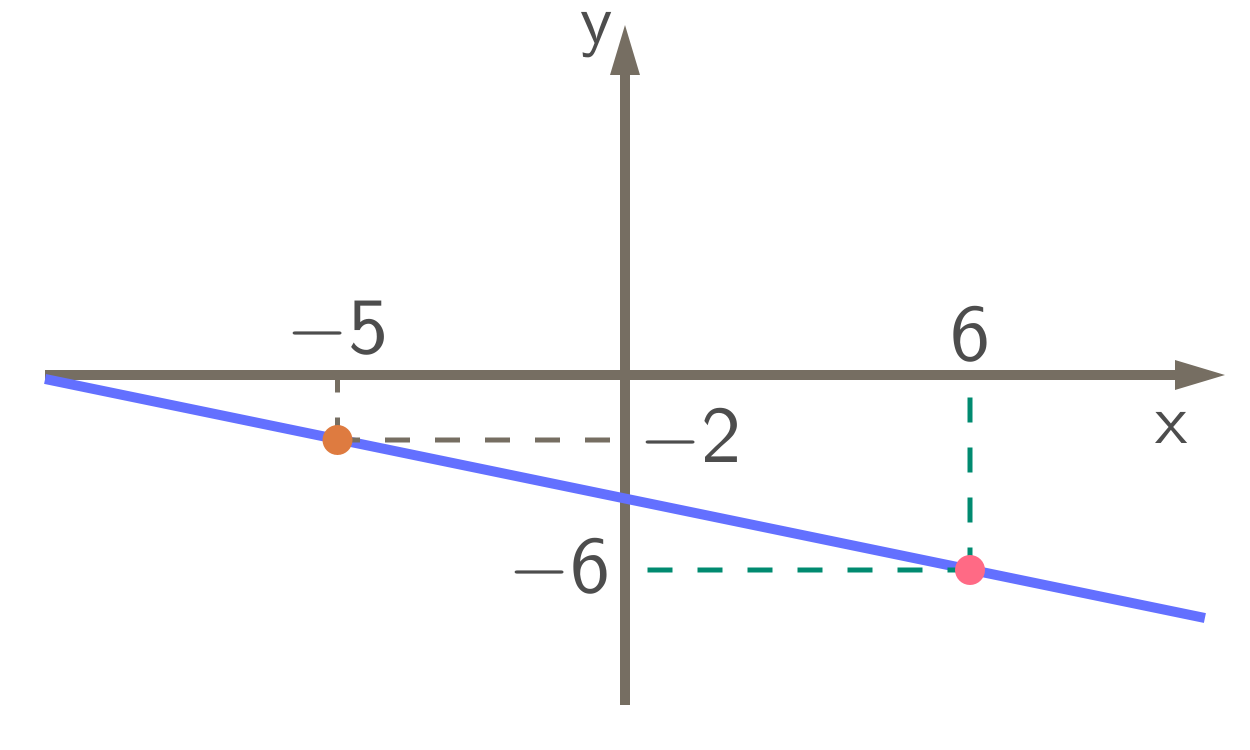
\includegraphics[width=0.6\linewidth]{img_06_1.png}\par}} \\
\exd{07}{Encontre o coeficiente angular da reta:\par {\centering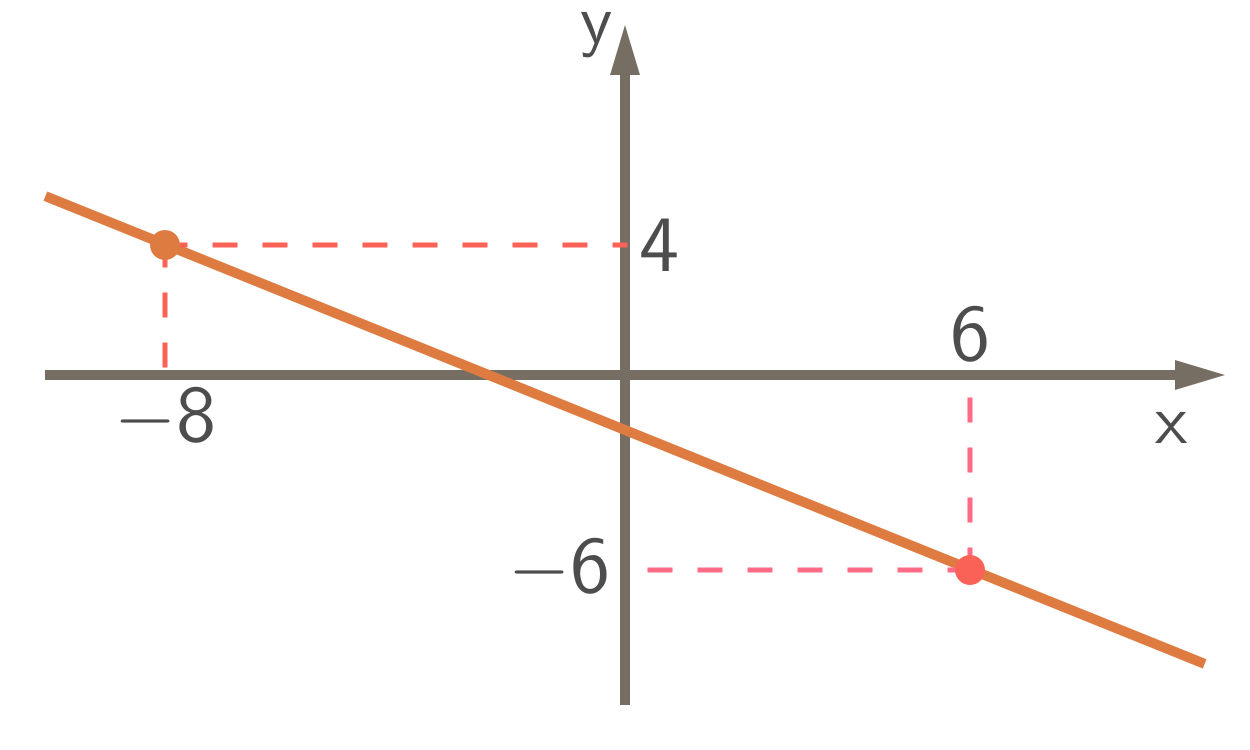
\includegraphics[width=0.6\linewidth]{img_07_1.png}\par}} &
\exd{08}{Encontre o coeficiente angular da reta:\par {\centering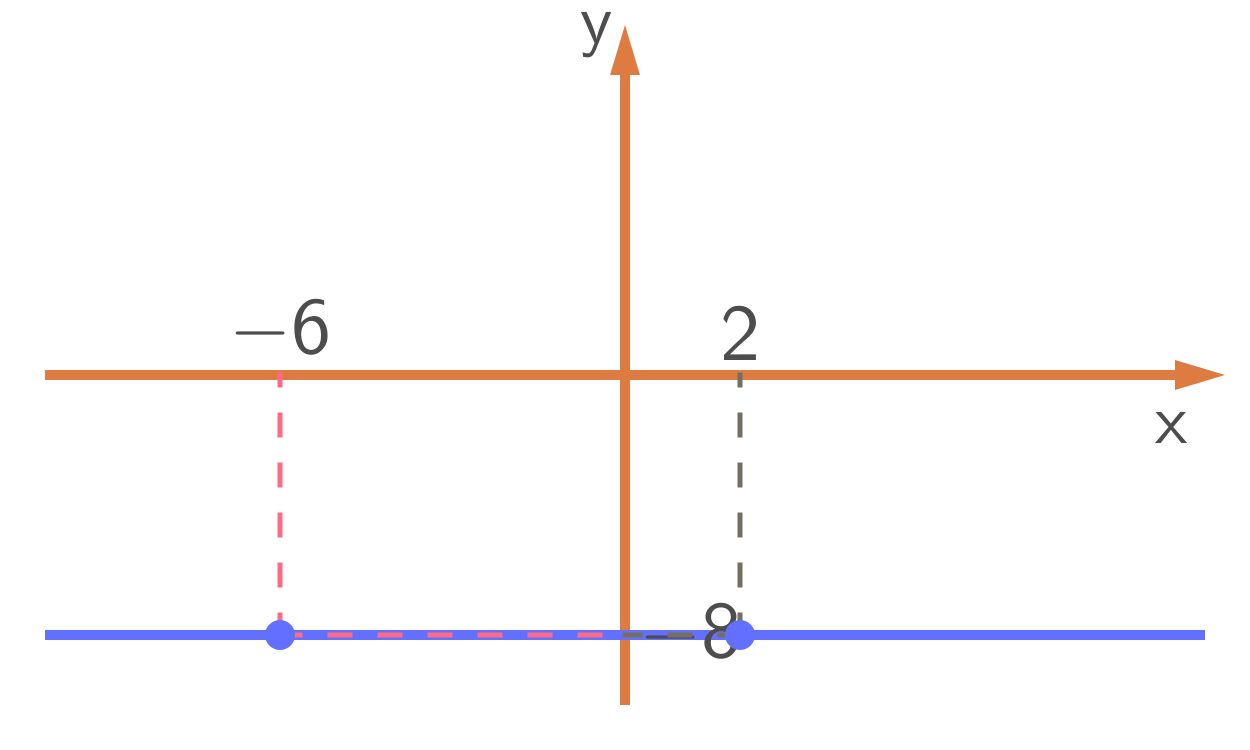
\includegraphics[width=0.6\linewidth]{img_08_1.png}\par}} \\
\end{tblr}

\newpage

\listheader{Função Afim}{Nível III}{Matemática · Intermediário}{Resolva as questões abaixo mostrando o desenvolvimento completo.}

\noindent
\begin{tblr}{
  width    = \textwidth,
  colspec  = {X|[1.5pt,sepcolor]X},
  columns  = {colsep=0pt, leftsep=7pt, rightsep=7pt},
  column{1} = {leftsep=0pt},
  column{2} = {rightsep=0pt},
  rows     = {ht=11.7cm, valign=t, rowsep=0pt},
}
\exd{09}{Determine os valores de \(x\) para os quais \(f(x) = -5x + 20 < 0\).} &
\exd{10}{Encontre o coeficiente angular da reta:\par {\centering\includegraphics[width=0.6\linewidth]{img_10_1.png}\par}} \\
\exd{11}{Encontre o valor de b:  \( f(x)=\dfrac{-6}{10}x+b \)\par {\centering\includegraphics[width=0.6\linewidth]{img_11_1.png}\par}} &
\exd{12}{Encontre o valor de b:  \( f(x)=\dfrac{4}{4}x+b \)\par {\centering\includegraphics[width=0.6\linewidth]{img_12_1.png}\par}} \\
\end{tblr}

\newpage

\listheader{Função Afim}{Nível III}{Matemática · Intermediário}{Resolva as questões abaixo mostrando o desenvolvimento completo.}

\noindent
\begin{tblr}{
  width    = \textwidth,
  colspec  = {X|[1.5pt,sepcolor]X},
  columns  = {colsep=0pt, leftsep=7pt, rightsep=7pt},
  column{1} = {leftsep=0pt},
  column{2} = {rightsep=0pt},
  rows     = {ht=11.7cm, valign=t, rowsep=0pt},
}
\exd{13}{Encontre o coeficiente angular da reta:\par {\centering\includegraphics[width=0.6\linewidth]{img_13_1.png}\par}} &
\exd{14}{Determine os valores de \(x\) para os quais \(f(x) = x - 2 > 0\).} \\
\exd{15}{Encontre o valor de b:  \( f(x)=\dfrac{13}{11}x+b \)\par {\centering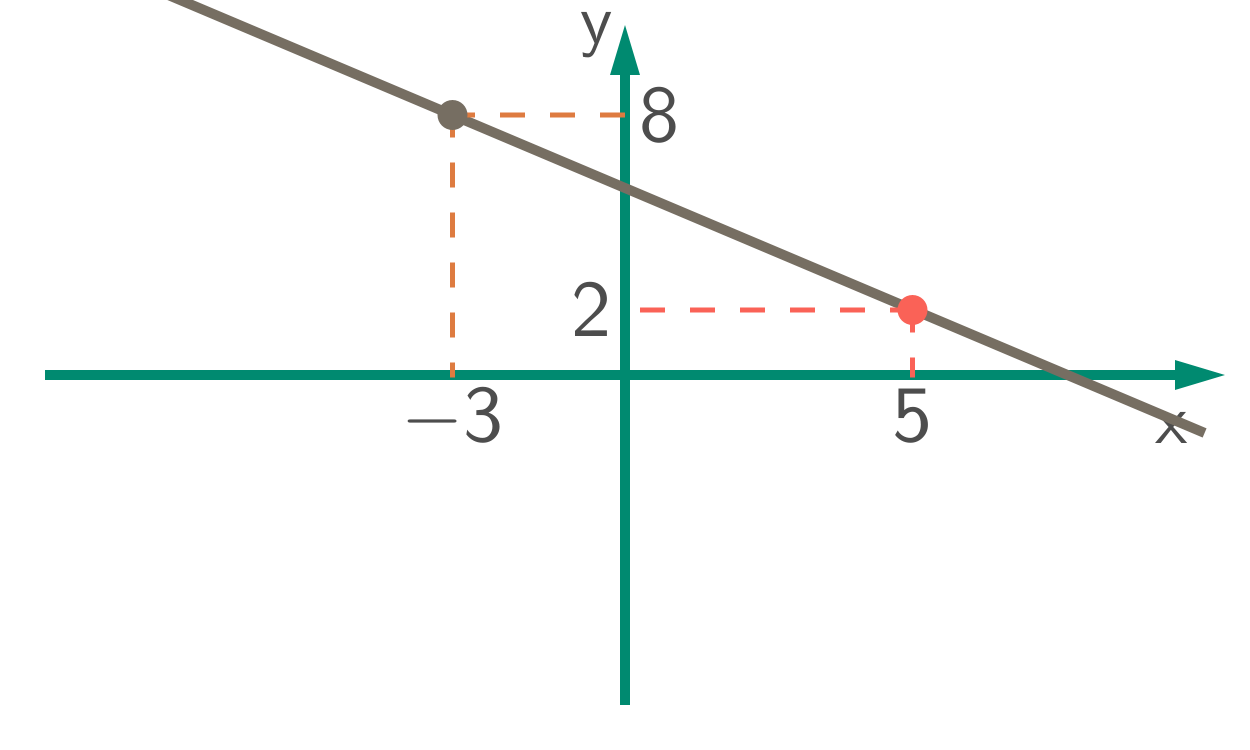
\includegraphics[width=0.6\linewidth]{img_15_1.png}\par}} &
\exd{16}{Determine os valores de \(x\) para os quais \(f(x) = -2x - 4 < 0\).} \\
\end{tblr}

\clearpage

\listheader{Função Afim}{Nível III}{Matemática · Intermediário}{Gabarito — Resolução comentada}

\DefTblrTemplate{caption}{default}{}
\DefTblrTemplate{conthead}{default}{}
\DefTblrTemplate{conthead-text}{default}{}
\DefTblrTemplate{contfoot}{default}{}
\DefTblrTemplate{contfoot-text}{default}{}
\begin{longtblr}[label=none]{
  width    = \textwidth,
  colspec  = {X|[1.5pt,sepcolor]X},
  columns  = {colsep=0pt, leftsep=7pt, rightsep=7pt},
  column{1} = {leftsep=0pt},
  column{2} = {rightsep=0pt},
  rows     = {valign=t, rowsep=0pt},
}
\resd{01}{Primeiro encontramos o zero \(x_0\): \(\\\)\(4x + 24 = 0\) \(\\\)\(x_0 = -\dfrac{24}{4} = \mathbf{-6}\) \(\\\)A função é crescente (\(a > 0\)), portanto: \(\\\)\(f(x) > 0\) quando \(\mathbf{x > -6}\)} &
\resd{02}{Coeficiente angular \(a\): \(\\\)\(a=\dfrac{\Delta y}{\Delta x} = \dfrac{y_B - y_A}{x_B-x_A}\\a= \dfrac{-4 - 6}{2-(-3)}= \dfrac{-4-6}{2+3}=\dfrac{-10}{5}=-2\) \(\\\)Coeficiente linear \(b\) usando \(A = (-3,\ 6)\): \(\\\)\(6 = -2 \cdot \left(-3\right) + b\) \(\\\)\(b = 6 - 6 = \mathbf{0}\) \(\\\)Logo \(f(x) = -2x\): \(\\\)\(f(4) = -2 \cdot 4 + 0 = -8 = \mathbf{-8}\)} \\
\resd{03}{O coeficiente linear  \(b\)  pode ser calculado por: \(\\ \)\(y=\dfrac{-4}{10}x + b \\ \)Considerando o ponto (-4,7),  temos: \(\\ \)\(7 = -\dfrac{4}{10} \cdot -4 +b \\7 = \dfrac{8}{5} +b \\-b = \dfrac{8}{5} -7 = -\dfrac{27}{5} \\b = \dfrac{27}{5} \)} &
\resd{04}{Primeiro encontramos o zero \(x_0\): \(\\\)\(-3x - 15 = 0\) \(\\\)\(x_0 = -\dfrac{15}{3} = \mathbf{-5}\) \(\\\)A função é decrescente (\(a < 0\)), portanto: \(\\\)\(f(x) > 0\) quando \(\mathbf{x < -5}\)} \\
\resd{05}{Primeiro encontramos o zero \(x_0\): \(\\\)\(x - 1 = 0\) \(\\\)\(x_0 = \mathbf{1}\) \(\\\)A função é crescente (\(a > 0\)), portanto: \(\\\)\(f(x) < 0\) quando \(\mathbf{x < 1}\)} &
\resd{06}{O coeficiente linear  \(b\)  pode ser calculado por: \(\\ \)\(y=\dfrac{4}{12}x + b \\ \)Considerando o ponto (-7,-7),  temos: \(\\ \)\(-7 = \dfrac{4}{12} \cdot -7 +b \\-7 = -\dfrac{7}{3} +b \\-b = -\dfrac{7}{3} +7 = \dfrac{14}{3} \\b = -\dfrac{14}{3} \)} \\
\resd{07}{Dados os pontos  \(A=(-4,-7)\)  e \(B=(5,3)\), temos que o coeficiente angular  \(a\)  é calculado por: \(\\ \)\(a=\dfrac{\Delta y}{\Delta x} = \dfrac{y_B - y_A}{x_B-x_A}\\a= \dfrac{3 - (-7)}{5-(-4)}= \dfrac{3+7}{5+4}=\dfrac{10}{9}\)} &
\resd{08}{Dados os pontos  \(A=(-2,3)\)  e \(B=(8,-8)\), temos que o coeficiente angular  \(a\)  é calculado por: \(\\ \)\(a=\dfrac{\Delta y}{\Delta x} = \dfrac{y_B - y_A}{x_B-x_A}\\a= \dfrac{-8 - 3}{8-(-2)}= \dfrac{-8-3}{8+2}=\dfrac{-11}{10}\)} \\
\resd{09}{Primeiro encontramos o zero \(x_0\): \(\\\)\(-5x + 20 = 0\) \(\\\)\(x_0 = \dfrac{20}{5} = \mathbf{4}\) \(\\\)A função é decrescente (\(a < 0\)), portanto: \(\\\)\(f(x) < 0\) quando \(\mathbf{x > 4}\)} &
\resd{10}{Dados os pontos  \(A=(-5,-6)\)  e \(B=(7,-5)\), temos que o coeficiente angular  \(a\)  é calculado por: \(\\ \)\(a=\dfrac{\Delta y}{\Delta x} = \dfrac{y_B - y_A}{x_B-x_A}\\a= \dfrac{-5 - (-6)}{7-(-5)}= \dfrac{-5+6}{7+5}=\dfrac{1}{12}\)} \\
\resd{11}{O coeficiente linear  \(b\)  pode ser calculado por: \(\\ \)\(y=\dfrac{-6}{10}x + b \\ \)Considerando o ponto (-7,8),  temos: \(\\ \)\(8 = -\dfrac{6}{10} \cdot -7 +b \\8 = \dfrac{21}{5} +b \\-b = \dfrac{21}{5} -8 = -\dfrac{19}{5} \\b = \dfrac{19}{5} \)} &
\resd{12}{O coeficiente linear  \(b\)  pode ser calculado por: \(\\ \)\(y=\dfrac{4}{4}x + b \\ \)Considerando o ponto (-2,3),  temos: \(\\ \)\(3 = \dfrac{4}{4} \cdot -2 +b \\3 = -2 +b \\-b = -2 -3 = -5 \\b = 5 \)} \\
\resd{13}{Dados os pontos  \(A=(-4,-6)\)  e \(B=(5,-6)\), temos que o coeficiente angular  \(a\)  é calculado por: \(\\ \)\(a=\dfrac{\Delta y}{\Delta x} = \dfrac{y_B - y_A}{x_B-x_A}\\a= \dfrac{-6 - (-6)}{5-(-4)}= \dfrac{-6+6}{5+4}=0=0\)} &
\resd{14}{Primeiro encontramos o zero \(x_0\): \(\\\)\(x - 2 = 0\) \(\\\)\(x_0 = \mathbf{2}\) \(\\\)A função é crescente (\(a > 0\)), portanto: \(\\\)\(f(x) > 0\) quando \(\mathbf{x > 2}\)} \\
\resd{15}{O coeficiente linear  \(b\)  pode ser calculado por: \(\\ \)\(y=\dfrac{13}{11}x + b \\ \)Considerando o ponto (-6,-5),  temos: \(\\ \)\(-5 = \dfrac{13}{11} \cdot -6 +b \\-5 = -\dfrac{78}{11} +b \\-b = -\dfrac{78}{11} +5 = -\dfrac{23}{11} \\b = \dfrac{23}{11} \)} &
\resd{16}{Primeiro encontramos o zero \(x_0\): \(\\\)\(-2x - 4 = 0\) \(\\\)\(x_0 = -\dfrac{4}{2} = \mathbf{-2}\) \(\\\)A função é decrescente (\(a < 0\)), portanto: \(\\\)\(f(x) < 0\) quando \(\mathbf{x > -2}\)} \\
\end{longtblr}

\end{document}
